\chapter{Ontwikkeling cross platforme mobiele applicatie}
\label{ch:ontwikkelingcrossplatformapp}
\section{Analyse van het project}
Als start van het project werd er een analyse gemaakt door de co-promotor van de functionele requirements.

Deze analyse bestaat uit het sturen van een query naar de databank die draait in een webservice.
Op deze manier worden de gegevens omgezet naar JSON \footnote{De afkorting staat voor
JavaScript Object Notation \cite{inleidingtotjson2017}}, een makkelijk genereerbaar gegevensformaat dat eenvoudig te lezen is voor toepassingen en vaak gebruikt wordt in webservice.  Het grote voordeel van JSON
is dat het makkelijk leesbaar/te genereren is voor/door toepassingen.

\section{Ontwikkeling van de ASP.NET MVC Web api}
De ASP.NET MVC Web api heeft in deze toepassing 2 functies. De REST API heeft als functie gebruikers zich te laten
authenticeren bij het Active Directory domein van de Gentse Politie. Nadien levert de REST API de gegevens die binnen
de applicatie nodig zijn voor de gebruikers. Deze authenticatie gebeurt aan de hand van tokens die een bepaalde tijd geldig zijn (in deze casus een week) \citep{authenticatemvcapplication2017}. Nadien moet de gebruiker zich opnieuw authenticeren aan de hand van de inloggegevens. Dit om opnieuw een
token met geldigheid van 1 week te verkrijgen. De tokens zijn verplicht toe te voegen aan de request. Indien dit niet gebeurt, stuurt
de server een antwoord dat men geen toegang heeft tot de aangevraagde resources. De schematische voorstelling van deze techniek,
kan u terugvinden op de volgende pagina.

\begin{figure}[ht!]
\centering
\caption{Token-authenticatie met ASP.NET MVC Web api}
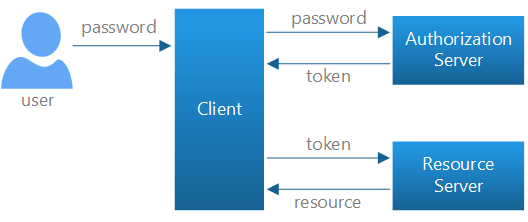
\includegraphics[width=90mm]{./img/authentication.png}
\end{figure}

\section{Ontwikkeling van de cross platforme mobiele applicatie}
\subsection{Gedeelde code}
Om de applicaties zo efficiënt mogelijk te ontwikkelen, wordt er code gedeeld tussen de deelprojecten van de 3 mobiele
platformen. Concreet gaat dit over de code die nodig is voor het ophalen van de gegevens uit de webservice gemeenschappelijk
gesteld wordt voor zowel het Android-, als het iOS- en Windowsphone-project. Ook het domeinmodel wordt gemeenschappelijk
gedefinieërd voor de drie mobiele applicaties. In het project gebeurd dit door in ieder deelproject een referentie toe te voegen
naar het gemeenschappelijke project.

\subsubsection{Code om data op te halen uit de REST-api}
De code die volledig gedeeld wordt omwille van de efficientië, is de code om de data op te halen uit de REST-service.
Hieronder vindt u het voorbeeld dat als basis diende voor de ontwikkeling van de cross platforme mobiele applicatie.
De volledige code met uitgebereide stappen om dit voorbeeld te ontwikkelen is beschikbaar op \citet{buildappwithnativeuiusingxamarininvisualstudio2017}.

Ter voorbereiding van de logica om data uit een REST-api op te halen hebben we een klasse nodig die de entiteit uit het
domein van de toepassing voorziet. In dit geval gaat het om de klasse Persoon met onder andere de velden Voornaam, Familienaam, Geslacht.
\newpage
\begin{lstlisting}
namespace MobileApp
{
  public class Persoon
  {
    public string Voornaam {get; set;}
    public string Familienaam {get; set;}
    public string Geslacht {get; set;}
  }
}
\end{lstlisting}
Nu deze domeinklasse gedefinieërd is, kunnen we verdergaan met een klasse aan te maken voor het effectief ophalen van
gegevens uit de REST-service. Hierbij is het belangrijk om op te merken dat deze code asynchroon op de main-thread van de
applicatie wordt uitgevoerd. Voorlopig ziet de klasse er als volgt uit:
\begin{lstlisting}
using System.Threading.Tasks;
using Newtonsoft.Json;
using System.Net.Http;
namespace MobileApp
{
  public class DataService
  {
    public async Task<string> getData(string queryString)
    {
      // Implementatie DataService.getData(string queryString)
    }
  }
}
\end{lstlisting}
Nu we de methode gedefinieërd hebben, kunnen we deze verder implementeren.
Deze implementatie zal bestaan uit 2 delen. In eerste instantie wordt de data opgehaald uit de REST-api, nadien zal de opgehaald data
omgevormd worden tot objecten van het type ''Persoon''. Dit type is hierboven reeds gedefinieërd.

De volgende code die we toevoegen aan de klasse ''DataService'' onder ''// Implementatie DataService.getData(string queryString)", is de code om de data als JSON binnen te halen.
Hiervoor moet er eerst een instantie van de klasse HttpClient (uit de namespace System.Net.Http) aangemaakt worden.
\begin{lstlisting}
  HttpClient client = new HttpClient();
\end{lstlisting}
\newpage
Nu de instantie van HttpClient geïnstanceerd is, kan deze gebruikt worden om data op te halen bij de webservice.
Het ophalen van de data gebeurt aan de hand van onderstaande code:
\begin{lstlisting}
  namespace MobileApp
  {
    // Imports statements

    public class DataService
    {
      public async List<Person> getData(string queryString)
      {
        // een instantie van de klasse HttpClient aanmaken
        HttpClient client = new HttpClient();

        // data ophalen uit de webservice
        HttpResponseMessage response = await client.GetAsync(queryString);

        // data converteren naar persoon-objecten
        List<Person> personen = JsonConvert.DeserializeObject<List<Person>>(response);

        // persoon-objecten teruggeven
        return personen;
      }
    }
  }
\end{lstlisting}



\subsection{Platform specifieke code}
De deelprojecten voor de drie mobiele applicaties bestaat enerzijds uit de definitie van de schermen voor de mobiele applicaties.
Deze definitie gebeurt in xml voor Android, xaml voor windowsphone en storyboard voor iOS.

Anderzijds is ook de code die de gebruikersevent van de GUI opvangen. In deze code wordt er vervolgens een request gestuurd naar
de api voor authenticatie en data.
